\documentclass[11pt]{article}

\usepackage[margin=2.5cm]{geometry}
\usepackage{graphicx}
\usepackage{listings}
\usepackage{xpatch}
\usepackage{color}
\usepackage{amsmath}
\usepackage[spanish]{babel}
\usepackage[utf8]{inputenc}
\usepackage{url}

\usepackage[round]{natbib}

\begin{document}
	{	\centering
		\scshape
		\LARGE
		Universidad de los Andes
		
		\large
		Departamento de F\'isica
		
		\vspace{1cm}
		
		Propuesta de Proyecto Microscop\'ia Moderna
		
		Microsc\'opio de escaneo laser
		
		\normalsize
		Juan Barbosa
		
	}
	
	\section{Introducci\'on}		
		La microscop\'ia de escaneo laser es una t\'ecnica de microscop\'ia en la cual se hace incidir luz sobre una peque\~na parte de un objeto, y se cuantifica la reflexi\'on de la misma. En ese sentido hace parte de las t\'ecnicas de luz reflejada. Dado que el punto donde se concentra la luz es relativamente peque\~no respecto a el tama\~no de la muestra, es necesario samplear la reflexi\'on en los ejes $x$ y $y$.
		
		Experimentalmente la parte \'optica se compone de un \textit{beam splitter} y uno o m\'as lentes para enfocar el haz de luz. 	El microscópio confocal es el mayor exponente de esta técnica de microscopía, el cual además de los elementos observados en la figura cuenta con dos \textit{pinholes} los cuales permiten realizar seccionamiento estructural sobre la muestra.
		
		\begin{figure}[h]
			\centering
			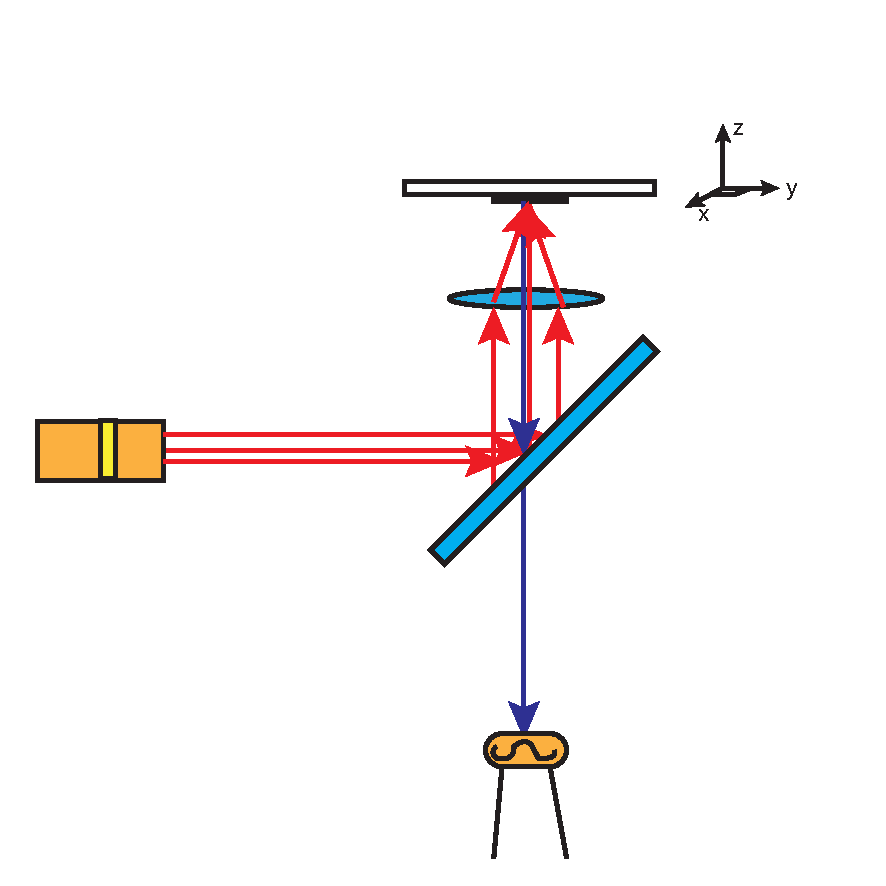
\includegraphics[width=0.35\linewidth]{beam.pdf}
			\caption{El haz de luz proveniente del laser, se refleja y se enfoca usando un lente. El rayo incide sobre la muestra, y la luz reflejada es captada por un detector.}
		\end{figure}
	
	\section{Objetivos}
		\begin{enumerate}
			\item Construcci\'on de un microsc\'opio de escaneo laser usando materiales de f\'acil acceso comercial.
			\item Adquirir datos con diferentes muestras.
			\item Mantener el presupuesto bajo, la electr\'onica s\'imple y el c\'odigo legible. Se espera que el proyecto a futuro sirva de forma pedag\'ogica, para las ciencias computacionales y la electr\'onica.
		\end{enumerate}
	
	\section{Metodolog\'ia}
		El sistema \'optico necesario para la implementaci\'on del proyecto se encuentra en su totalidad contenida en los m\'odulos de lectura (y escritura) de medios digitales tales como CD, DVD y Blu-Ray. De estos tres sistemas el de menor longitud de onda es el Blu-Ray, sin embargo el sistema \'optico se encuentra minimizado, dificultando el acceso a las partes relevantes. Por esta raz\'on se opt\'o por el sistema \'optico de los CD's, los cuales ya se encuentran adquiridos y corresponden con la referencia \texttt{KSS-213B}.
		
		En estos sistemas se realizaron cambios de los l\'aseres infrarrojos por rojos de acceso comercial local. La etapa de detecci\'on tambi\'en se modific\'o, reemplazando el fotodiodo por un fotoresistor, sin embargo esta etapa aún no se encuentra implementada en su totalidad, dado que es necesaria una etapa de resta al fondo y amplificaci\'on. Los sistemas de CD usados cuentan con dos bobinas internas para controlar el enfoque ($z$) y el movimiento en una direcci\'on $x$ \'o $y$. Estos movimientos son lo suficientemente peque\~nos para seguir los datos grabados sobre la superficie de un cd ($\approx 1\mu$m). De los dos sistemas \'opticos con los que se cuenta, el primero tiene las funciones de enfoque y movimiento en $x$, mientras el otro s\'olo se mueve en $y$.
		
		El microsc\'opio en su interior cuenta con un microcontrolador \texttt{Atmega 328}, el cual se encarga de realizar los movimientos en $x$ y $y$, obtener los datos y enviarlos por puerto USB a un computador usando un protocolo UART. Esta etapa ya se encuentra implementada. En el computador los datos son recibidos y graficados, al finalizar el projecto se espera contar con una libreria en Python para simplificar el acceso a los datos, sin perder de vista el hecho que el microsc\'opio ser\'a manejado con c\'odigo y no con una interfaz gr\'afica, esto con el objetivo de motivar la computaci\'on a nivel general.
		
		\begin{figure}[h]
			\centering
			\includegraphics[width=0.7\linewidth]{breadboard.jpg}
			\caption{Circuito actual. (1) Microcontrolador. (2) Puente H, etapa de potencia para los motores. (3) Sistema \'optico principal con laser y movimiento en $x$. (4) Sistema \'optico con movimiento en $y$. (5) Comunicaci\'on UART.}
		\end{figure}
	
		El enfoque se llevará a cabo sampleando un único punto para distintas alturas. Al graficar las intensidades el máximo corresponderá con la altura donde la muestra se encuentra enfocada (luz incidiendo en una menor área pero con mayor intensidad), para esto se usa derivación numérica.
		\begin{equation}
			df_i = \dfrac{f_{i+1} - f_{i-1}}{2\Delta h} \qquad \text{$f_i$ corresponde con el dato i-ésimo. Estará enfocada si $-\epsilon < df_i < \epsilon$.}
		\end{equation}
		
		Finalmente se prevee una complicación en el manejo de las muestras, puesto que hasta el momento no se ha considerado un montaje para facilitar su ubicación en el microscópio.
		
	\subsection{Resultados preliminares}
	Los resultados preliminares muestran la forma de escanéo de un blanco (objetivo vacío) con condiciones de luz estables en el cuarto donde se realiza el montaje.
	\begin{figure}[h]
		\centering
		\begin{tabular}{cc}
			\includegraphics[width=0.3\linewidth]{data1.png} &
			\includegraphics[width=0.3\linewidth]{data2.png}
		\end{tabular}
		\caption{Barrido, observado en el computador. La escala corresponde a 10-bits.}
	\end{figure}

	Usando una factura en papel térmico se realiza una la primera prueba con una muestra reflectiva, si bien la imágen se ve ruidosa, se debe en parte a la poca estabilidad en la iluminación ambiente al tomar los datos.
	\begin{figure}[h]
		\centering
		\includegraphics[width=0.7\linewidth]{complete.pdf}
		\caption{Primera línea horizontal de la letra E en una factura.}
	\end{figure}

	Es importante mencionar que la imagen anterior corresponde con resultados obtenidos sin amplificación y eliminación del fondo, por lo cual se usan menos de 7 bits de 10 disponibles.
	\newpage
	
	\section{Plan B (Colaboración)}
	Otra opción para realizar el movimiento en las tres dimensiones es el uso de 2 motores de paso y un stepper. Los primeros usados en los ejes $x$ y $y$, y el último en $z$. Estos ya se encuentran adquiridos (\texttt{Neocene 2T3542232} y \texttt{TowerPro SG90}). El número de pasos requeridos para dar una vuelta es de $n_0 = 96$ (\texttt{Neocene 2T3542232}).
	\begin{equation}
		\theta_0 = \dfrac{2\pi}{n_0}= 0.06545 \text{ rad} \qquad \text{\'angulo por paso}
	\end{equation}
	\begin{equation}
		s_0 = r\theta_0 = 654.5 \mu\text{m} \qquad \text{movimiento longitudinal por paso, suponiendo r = 1 cm}
	\end{equation}
	
	Se propone entonces la construcción de un moto reductor con una relación $\alpha$:1, con $\alpha = 71$. El movimiento longitudinal de busca realizar usando una correa de distribución (ya adquirida) con un montaje análogo al mostrado en la siguiente figura.
	\begin{equation}
		s = \dfrac{r\theta_0}{\alpha} \approx 9.2 \mu\text{m}
	\end{equation}
	
	\begin{figure}[h]
		\centering
		\begin{tabular}{ccc}
			\includegraphics[width=0.4\linewidth]{correa1.jpg} &
			\includegraphics[width=0.4\linewidth]{correa2.jpg} &
		\end{tabular}
		\caption{Propuesta para movimientos longitudinales.}
	\end{figure}
	
	Este se encuentra en etapa de diseño y actualmente se realizan calibraciones.
	\begin{figure}[h]
		\centering
		\begin{tabular}{ccc}
			\includegraphics[width=0.3\linewidth]{rendered.png} &
			\includegraphics[width=0.3\linewidth]{rendered2.png} &
			\includegraphics[width=0.3\linewidth]{motoreductor.jpg}
		\end{tabular}
		\caption{Prototipo 1, Prototipo 2, impresión 3D prototipo 2.}
	\end{figure}
	
	\newpage
	\nocite{*}
	\bibliography{Bib}
	\bibliographystyle{plainnat}
	
	La totalidad de los archivos de soporte del proyecto, incluyendo este documento y los códigos para el funcionamiento del escaner láser como el movimiento longitudinal se encuentran en \url{https://github.com/jsbarbosa/miniscope}, y hacen parte del proyecto \texttt{Miniscope}.
\end{document}